
\newcommand{\annotate}[1]{{\color{figloop!75!black} \mathsf{#1}}}

Automating the generation of formal specifications for C code remains challenging due to the prevalence of complex language features such as loops, pointer manipulation, and data structures. Consider the code fragment shown in Fig.~\ref{fig:example}, which is adapted from a navigation component in an industrial control codebase. The code defines a struct \texttt{CheckCal} with three fields: an integer array \texttt{pkv[10]}, an integer field \texttt{len} representing the number of valid elements in the array, and an integer field \texttt{chksum} storing the sum of the array's elements. Function \texttt{foo} then invokes \texttt{CheckCalFun} on a \texttt{CheckCal} pointer \texttt{pIp}, with a verification goal annotated by \texttt{/*@ assert $\cdots$ */}. The callee function \texttt{CheckCalFun} takes a \texttt{CheckCal} pointer \texttt{pIp}, computes the sum of the \texttt{len} elements in the array \texttt{pkv} via a loop, and stores the result in the field \texttt{chksum} of \texttt{pIp}.
This example exhibits diverse features: complex data structures (structs, arrays and pointers), a loop with inductive operations over arrays, and pointer-induced aliasing and side effects.
Consequently, it faces the following challenges:
\begin{itemize}
  \item \textbf{Loop reasoning:}  
  The summation loop \texttt{for(; i<pIp->len; i++)} requires determining whether the initial state allows loop entry and, if the loop executes, establishing invariants strong enough to relate the partial sum to the processed prefix of the array.
  
  \item \textbf{Structs and Pointers:} The procedures access arrays and read and write struct fields through pointers, making it essential to account for aliasing and side effects in their specifications. For instance, the specification for function \texttt{CheckCalFun} must guarantee memory safety for dereferencing \texttt{pIp->pkv[i]}, precisely describe the write effect on \texttt{pIp->chksum}, and specify frame properties for fields of \texttt{pIp} that remain unchanged. 
  
  \item \textbf{Inductive predicates:}  
  Properties of arrays in loops, such as aggregate sums, are often most naturally expressed with inductive predicates or logic functions. Automatically writing such definitions in a verifier-friendly form and then proving the resulting annotations remains a central challenge for programs involving recursive operations or data structures.
\end{itemize}

\begin{figure*}
    \centering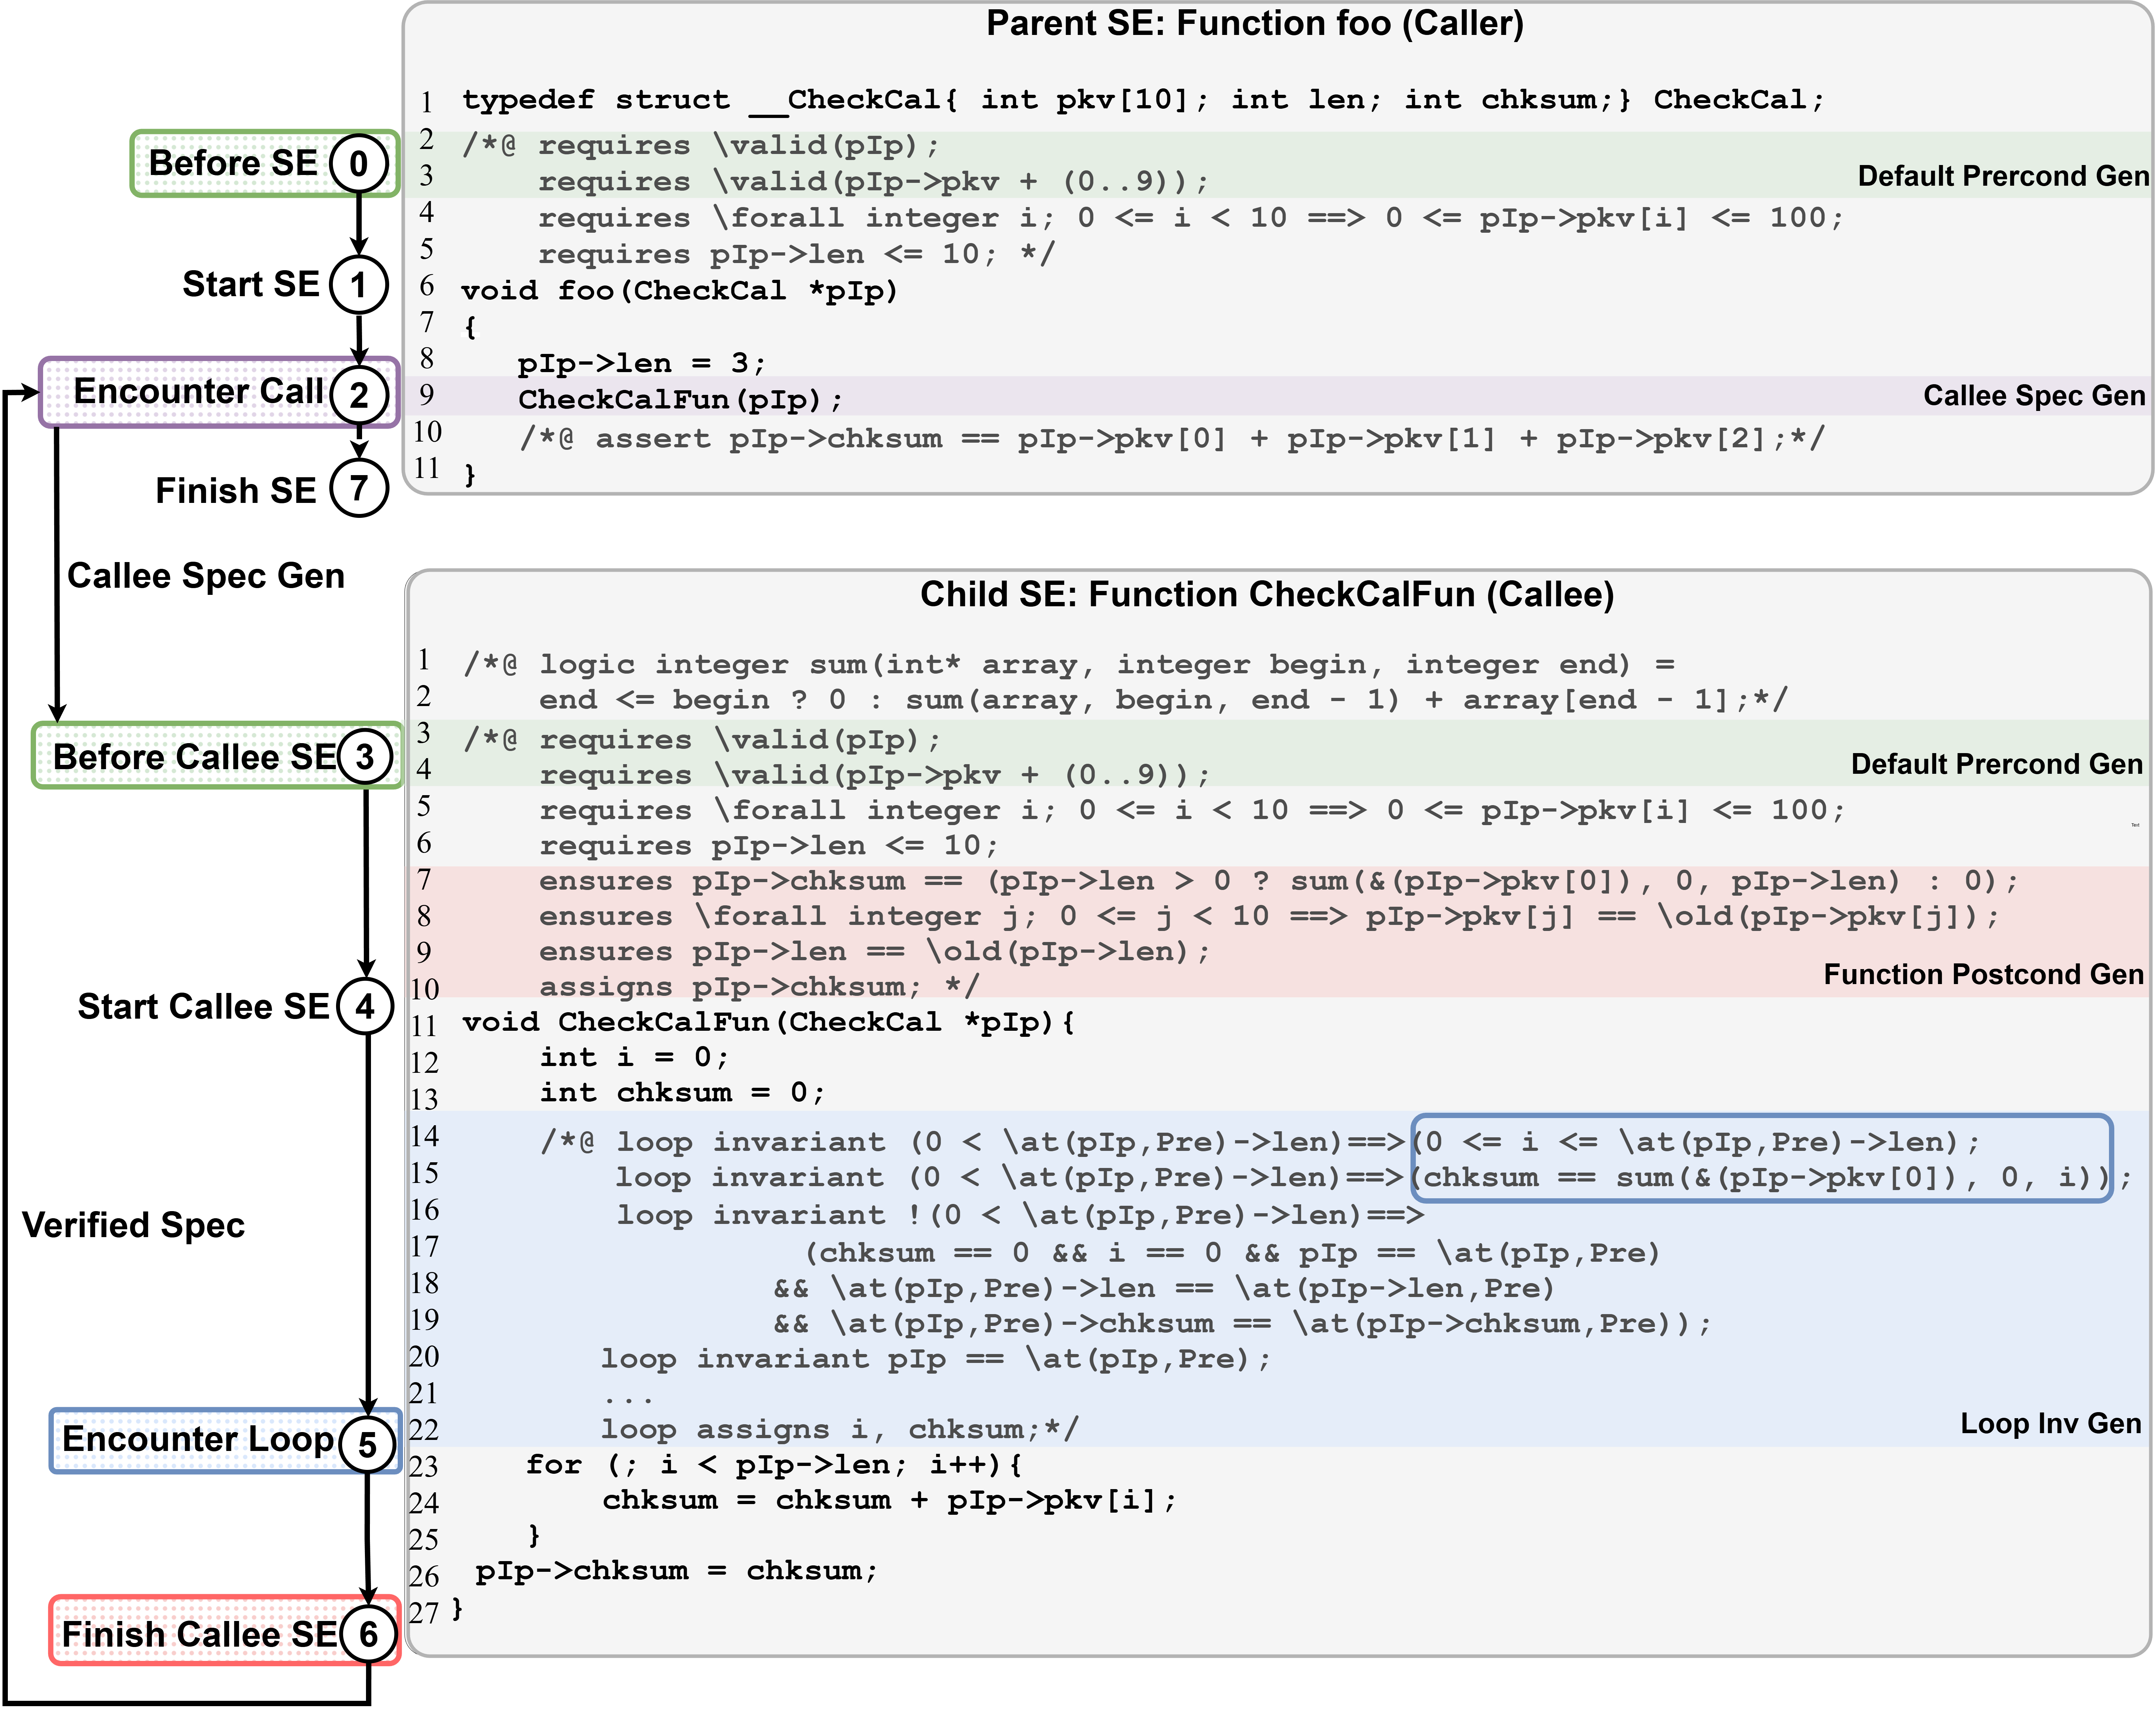
\includegraphics[width=0.9\textwidth]{images/example.png}
    \caption{Motivating Example}
    \label{fig:example}
\end{figure*}




As shown in Fig.~\ref{fig:example}, the code is annotated with the full ACSL specifications enclosed in $/*@ ... */$, including preconditions (beginning with \texttt{requires}), postconditions (beginning with \texttt{ensures}), loop invariants (beginning with \texttt{loop\ invariant}), and verification goals (beginning with \texttt{assert}).
Among these, the loop invariants, the default preconditions, and the postconditions are generated automatically by our tool \toolname, while the \texttt{assert} clause represents verification goals provided a priori, and the non-default preconditions shown on the designer-annotated \texttt{requires} lines of \texttt{CheckCalFun} in Fig.~\ref{fig:example} reflect additional requirements from the designers.


Before presenting our method, we attempted to generate the specification for this example using GPT-4o, Claude 3.7 Sonnet, and \autospec, given both the preconditions and the verification goal. The loop invariants they produced, shown below, were all found to be incorrect:

\[
\begin{array}{@{}l@{}}
\textsc{GPT-4o}\\
\texttt{loop invariant 0 <= i <= pIp->len;}\\
\texttt{loop invariant chksum ==}\\
\quad\texttt{\textbackslash sum(0, i-1, \textbackslash lambda integer k;}\\
\quad\texttt{pIp->pkv[k]);} \\
%\end{array}
%\]
%\[
%\begin{array}{@{}l@{}}
\\
\textsc{Claude 3.7 Sonnet}\\
\texttt{loop invariant 0 <= i <= pIp->len;}\\
\texttt{loop invariant chksum ==}\\
\quad\texttt{\textbackslash sum(integer k = 0; k < i; pIp->pkv[k]);}\\
\texttt{loop assigns i, chksum;}\\
\texttt{loop variant pIp->len - i;}
\\
\\
\autospec\\
\texttt{loop invariant 0 <= i <= pIp->len;} 
\end{array}
\]
\[
\begin{array}{@{}l@{}}
\texttt{loop invariant chksum ==}\\
\quad\texttt{\textbackslash sum(0, i-1, pIp->pkv);}\\
\texttt{loop invariant \textbackslash forall integer k;}\\
\quad\texttt{0 <= k < i ==> chksum >= pIp->pkv[k];}\\
\texttt{loop assigns i, chksum;}
\end{array}
\]

\DIFaddbegin
The failures highlight common limitations of pure LLM-based approaches. First, all three state the partial-sum relation but none guards the case in which the loop never executes (e.g., \texttt{pIp->len <= 0}): they assume loop entry, so even the well-formed clauses fail the base case. Even when we explicitly prompted GPT-4o to ``consider the case when the loop is not entered'', it still failed to produce the correct conditional invariant structure. Second, each tool invents a \emph{different} syntax for the array aggregate---\texttt{\textbackslash sum} with a lambda, with a quantified binder, or over a raw pointer---without defining it as an ACSL logic function; \texttt{\textbackslash sum} is not a construct that Frama-C/WP discharges by default, so these clauses are rejected as undefined.
\DIFaddend
 

 

 


 
